\documentclass[aspectratio=169]{beamer}
\usepackage{framed}
\usepackage{enumitem}
\usepackage{multicol}
\usepackage{fontspec}
\usepackage[english]{babel}
\usepackage{csquotes}
\usepackage{tikz}
\usepackage{tabu}

% General math package
\usepackage{amsmath}
\usepackage{amsfonts}
\usepackage{amssymb}
\usepackage{amsthm}
\usepackage{booktabs}
\usepackage{relsize}

\definecolor{violet}{HTML}{AA305C}
\definecolor{background}{HTML}{F9F9F6}
\definecolor{text}{HTML}{303030}

\setbeamertemplate{navigation symbols}{}
%\setbeamertemplate{footline}[frame number]

\setbeamercolor{title}{fg=violet}
\setbeamercolor{frametitle}{fg=violet}
\setbeamercolor{structure}{fg=violet}
\setbeamercolor{background canvas}{bg=background}
\setbeamercolor{normal text}{fg=text}

\usefonttheme{professionalfonts} % using non-standard fonts for beamer
\usefonttheme{serif} % default family is serif
%\setmainfont[Path=fonts/, UprightFont=*-R.ttf, ItalicFont=*-I.ttf]{GentiumPlus}
\setmainfont[Path=fonts/, UprightFont=*.ttf, ItalicFont=*-Italic.ttf, BoldFont=*-Bold.ttf]{Junicode}
%\setmainfont{STIX}
%\setmainfont{TeX Gyre Pagella}

% Tango color palette
\definecolor{butter1}{HTML}{FCE94F}
\definecolor{butter2}{HTML}{EDD400}
\definecolor{butter3}{HTML}{C4A000}
\definecolor{orange1}{HTML}{FCAF3E}
\definecolor{orange2}{HTML}{F57900}
\definecolor{orange3}{HTML}{CE5C00}
\definecolor{chocolate1}{HTML}{E9B96E}
\definecolor{chocolate2}{HTML}{C17D11}
\definecolor{chocolate3}{HTML}{8F5902}
\definecolor{chameleon1}{HTML}{8AE234}
\definecolor{chameleon2}{HTML}{73D216}
\definecolor{chameleon3}{HTML}{4E9A06}
\definecolor{skyblue1}{HTML}{729FCF}
\definecolor{skyblue2}{HTML}{3465A4}
\definecolor{skyblue3}{HTML}{204A87}
\definecolor{plum1}{HTML}{AD7FA8}
\definecolor{plum2}{HTML}{75507B}
\definecolor{plum3}{HTML}{5C3566}
\definecolor{scarletred1}{HTML}{EF2929}
\definecolor{scarletred2}{HTML}{CC0000}
\definecolor{scarletred3}{HTML}{A40000}
\definecolor{aluminium1}{HTML}{EEEEEC}
\definecolor{aluminium2}{HTML}{D3D7CF}
\definecolor{aluminium3}{HTML}{BABDB6}
\definecolor{aluminium4}{HTML}{888A85}
\definecolor{aluminium5}{HTML}{555753}
\definecolor{aluminium6}{HTML}{2E3436}

\newcommand{\backupbegin}{
   \newcounter{finalframe}
   \setcounter{finalframe}{\value{framenumber}}
}
\newcommand{\backupend}{
   \setcounter{framenumber}{\value{finalframe}}
}

\newcommand{\copyrightText}[2]{%
    {\par\scriptsize\color{aluminium4}\href{#2}{#1}}
}


\newcommand{\imageframe}[1]{%
    \setbeamertemplate{navigation symbols}{}%
    \begin{frame}[plain,noframenumbering]%
        \begin{tikzpicture}[remember picture,overlay]%
            \node[at=(current page.center)] {%
                \includegraphics[width=\paperwidth]{#1}%
            };%
        \end{tikzpicture}%
    \end{frame}%
}

\newcommand{\videoframe}[1]{%
    \begin{frame}[plain,noframenumbering]%
        \scalebox{.0001}{\texttt{\#!video:}\url{#1}}%
        \centering%
        \tiny\url{#1}%
    \end{frame}%
}



\title{Nengo Summerschool 2019}
\subtitle{Biologically Detailed Networks and Neuron Models}
\author{Peter Duggins, Andreas Stöckel}
\date{June 18, 2018}

\setbeamertemplate{footline}[frame number]

\renewcommand{\emph}[1]{{\color{violet}\textit{#1}}}
\setlist[itemize]{font=\color{violet},label=\textbullet} 

\AtBeginDocument{%
	\abovedisplayskip=6pt
	\abovedisplayshortskip=0pt
	\belowdisplayskip=6pt
	\belowdisplayshortskip=0pt
}

\begin{document} 

\begin{frame}[plain,noframenumbering]
	\centering\vspace{1cm}
	{\Large{\inserttitle}\\[0.25cm]}
	{\huge\color{violet}{\insertsubtitle}\\[0.75cm]}
	{\large{\insertauthor}\\[0.5cm]}
	
\includegraphics[height=2cm]{media/uwlogo.pdf}
	\raisebox{0.5cm}{
\includegraphics[height=1cm]{media/cnrg_logo.pdf}}\\[0.25cm]
	\insertdate
\end{frame}

\begin{frame}[plain,noframenumbering]
	{\centering\Huge\addfontfeature{LetterSpace=10.0}{OUTLINE}\\\color{aluminium3}\\}
	\large\vspace{-0.75cm}
	\setlist[enumerate]{font=\color{violet},labelindent=0cm,leftmargin=*,label=\Roman*,widest=III,align=right,labelsep=0.5cm}
	\begin{enumerate}
		\setlength{\itemsep}{0.5cm}
		\item<1-> \emph{Motivation \& Background}\\Why care about biological detail?
		\item<2-> \emph{Conductance-based $n$-LIF neurons} $\leftarrow$ Andreas\\How to computationally exploit nonlinear dendritic interaction
		\item<3-> \emph{Detailed NEURON Models and the NEF} $\leftarrow$ Peter\\How to integrate detailed neuron models into the NEF
		\item<4-> \emph{\texttt{nengo-bio} hands-on} $\leftarrow$ Andreas\\Build networks adhering to Dale's principle and exploit dendritic computation
	\end{enumerate}			
\end{frame}

\begin{frame}[noframenumbering,plain]
\centering
\Large\textsc{PART I}\\[0.5cm]
{\huge\color{violet}Motivation \& Background}
\end{frame}

\begin{frame}{Motivation --- \emph{Levels of Analysis}}
	\centering
	\vspace{1cm}
	\includegraphics<1>[scale=0.85]{media/levels_of_analysis_00.pdf}%
	\includegraphics<2>[scale=0.85]{media/levels_of_analysis_01.pdf}%
	\includegraphics<3>[scale=0.85]{media/levels_of_analysis_02.pdf}%
	\includegraphics<4>[scale=0.85]{media/levels_of_analysis_03.pdf}%
	\includegraphics<5>[scale=0.85]{media/levels_of_analysis_04.pdf}%
	\includegraphics<6>[scale=0.85]{media/levels_of_analysis_05.pdf}%
	\includegraphics<7>[scale=0.85]{media/levels_of_analysis_06.pdf}%
	\includegraphics<8>[scale=0.85]{media/levels_of_analysis_07.pdf}%
\end{frame}

\begin{frame}{Motivation --- \emph{Computational Power of Biological Neurons}}
	\vspace{0.25cm}
	\centering
	\includegraphics<1>[width=1\textwidth]{media/izhikevich_whichmod_figure1.pdf}
	\includegraphics<2>[width=1\textwidth]{media/izhikevich_whichmod_figure2.pdf}\\[0.25cm]
	{\footnotesize\color{aluminium4}Adapted from Izhikevich (2004), \textit{Which Model to Use for Cortical Spiking Neurons?}}
\end{frame}

\begin{frame}{Motivation --- \emph{Computational Power of Biological Neurons}}
	\begin{itemize}
		\setlength{\itemsep}{0.5cm}
		\item<1-> LIF model accounts for a fraction of the behaviour found in biological neurons
		\item<2-> \textbf{Questions:}\\
		\begin{itemize}
			\setlength{\itemsep}{0.3cm}
			\item In how far is the additional detail functionally \emph{relevant}?
			\item<3-> What is its role in terms of \emph{computation}?
			\item<4-> Can we \emph{harness} these details to perform computation?
		\end{itemize}
		\item<5-> \textbf{Example:}\\
		\begin{itemize}
			\setlength{\itemsep}{0.3cm}
			\item Excitatory and inhibitory channels interact nonlinearly.
			\item<6->[$\leadsto$] Can we exploit this nonlinearity systematically?
		\end{itemize}
	\end{itemize}
\end{frame}

%\begin{frame}{Motivation --- \emph{Neuromorphic Hardware}}
%	\begin{overlayarea}{\textwidth}{0.8\textheight}
%		\only<1->{\begin{columns}[b]
%			\column{0.5\textwidth}
%			\emph{(a)} Non-ideal model neurons implemented in neuromorphic hardware may be more efficient
%			\column{0.5\textwidth}
%			\emph{(b)} Some platforms (e.g.~BrainScaleS) implement more biologically detailed models
%		\end{columns}}
%		\only<2->{
%		\centering
%		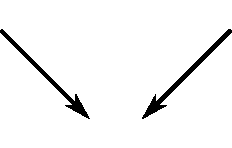
\includegraphics[scale=0.75]{media/diagonal_arrows.pdf}\\
%		\begin{minipage}{0.5\textwidth}
%			\centering
%			Methods presented here are applicable to neuromorphic hardware as well
%		\end{minipage}\\}
%		\only<3->{
%		
\includegraphics[scale=0.75]{media/down_arrow.pdf}\\
%		\begin{minipage}{0.5\textwidth}
%			Better utilization of neuromorphic hardware
%		\end{minipage}}
%	\end{overlayarea}
%\end{frame}

\begin{frame}{Motivation --- \emph{Recreating Idiosyncrasies of the Brain}}
	\centering
	\vspace{0.5cm}
	\includegraphics<1>[width=\textwidth]{media/motivation_idiosyncrasies_01.pdf}%
	\includegraphics<2>[width=\textwidth]{media/motivation_idiosyncrasies_02.pdf}%
	\includegraphics<3>[width=\textwidth]{media/motivation_idiosyncrasies_03.pdf}%
\end{frame}

\begin{frame}{Neurobiology --- \emph{Idealized \enquote{Textbook} Neuron}}
	\centering
	\vspace{1cm}
	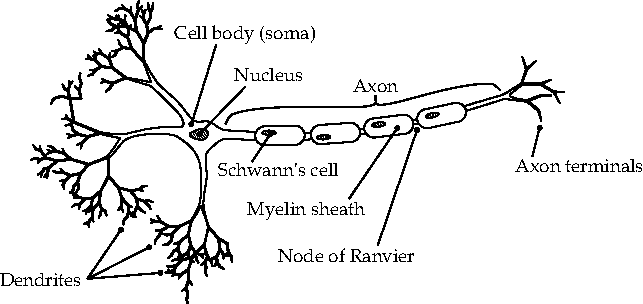
\includegraphics[width=0.8\textwidth]{media/neuron_sketch}\\[0.5cm]
	\begin{overlayarea}{\textwidth}{1cm}
		\centering
		\only<2->{
			{\color{violet}❶}
			Dendrites collect input $\longrightarrow$
			{\color{violet}❷}
			Integrated in soma $\longrightarrow$
			{\color{violet}❸}
			Output spikes travel along axon}
	\end{overlayarea}
\end{frame}

\begin{frame}{Neurobiology --- \emph{Neural Heterogeneity}}
	\begin{columns}
		\column{0.5\textwidth}
			\centering
			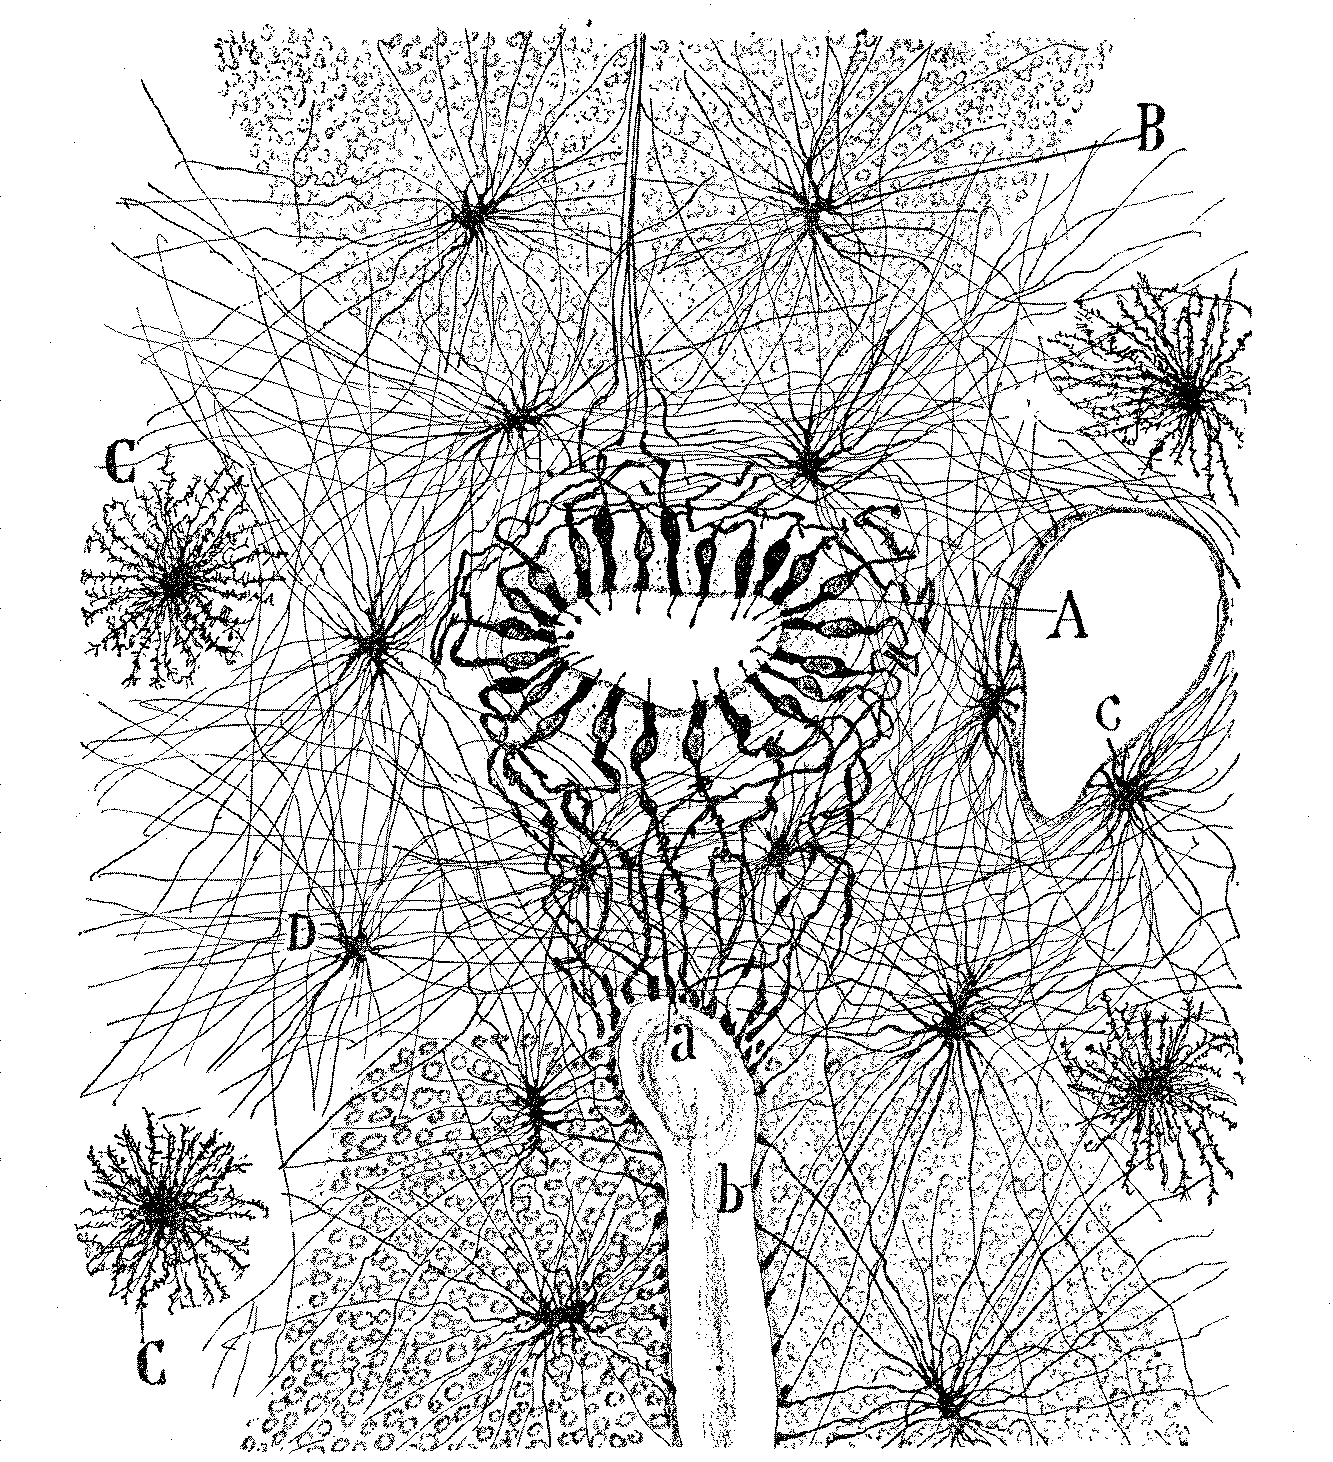
\includegraphics[width=\textwidth]{media/cajal_neuroglia.png}
		\column{0.5\textwidth}
			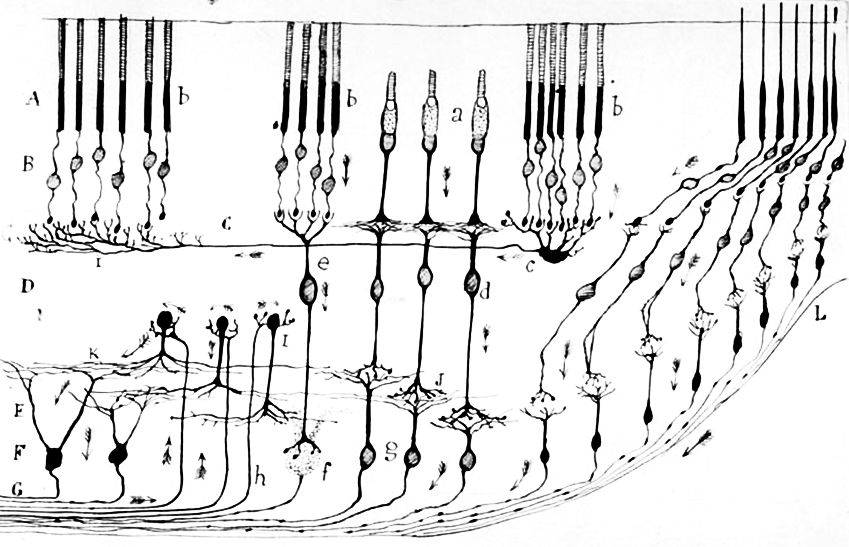
\includegraphics[width=0.8\textwidth]{media/cajal_retina.png}\\
			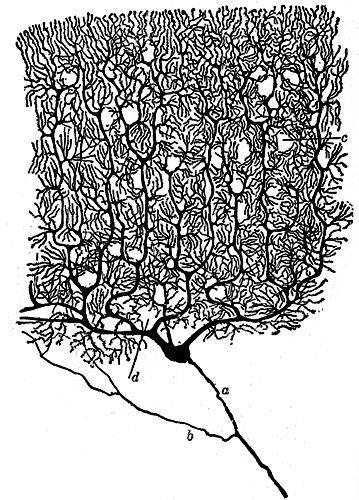
\includegraphics[width=0.4\textwidth]{media/cajal_purkinje.png}\\
			\vspace{-0.75cm}\begin{minipage}{6cm}{\raggedleft\footnotesize Drawings by\\Santiago Ramón y Cajal\\}\end{minipage}
	\end{columns}
\end{frame}


%\begin{frame}{Synapses --- \emph{Biophysics}}
%%\centering{How do neurons receive input signals from one another?}
%    \only<1>{
%    \begin{figure}
%      \centering
%      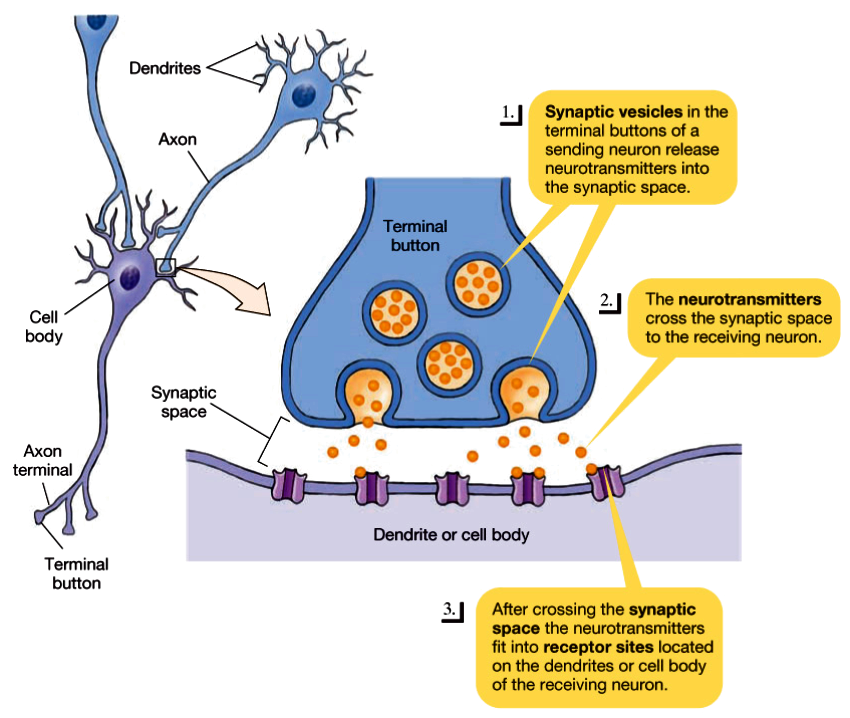
\includegraphics[height=0.925\textheight]{media/large_synapse.png}
%      % https://socratic.org/questions/how-do-impulses-travel-across-a-synapse
%    \end{figure}}
%%    \only<2>{
%%    \begin{figure}
%%      \centering
%%      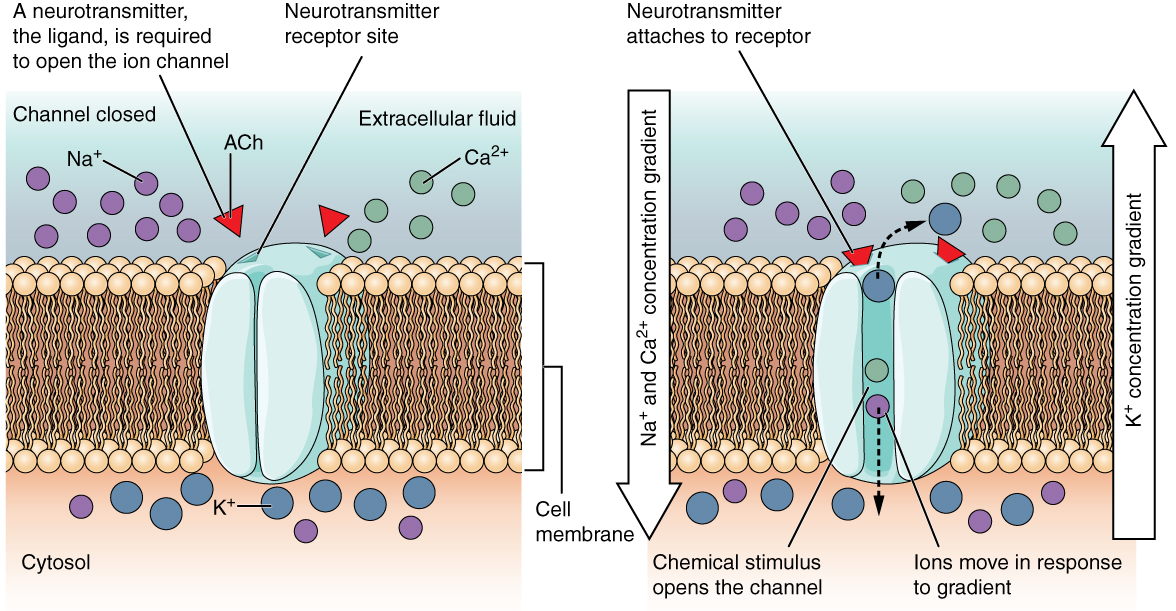
\includegraphics[height=0.8\textheight]{media/small_synapse.jpeg}
%%      % http://cbm.msoe.edu/crest/ePosters/2014alvernoPotassiumChannel.html
%%    \end{figure}}
%    % Figure here for current and voltage?
%    
%    % neurotransmitter random walk and receptor binding
%    % receptor kinetics and coupling with ion channels
%    % ion channel dynamics, current, and voltage
%    % receptor density and learning
%\end{frame}

%\begin{frame}{Synapses --- \emph{Conductance- and Current-Based Models}}
%	Mathematical formalism
%    \begin{itemize}
%      \item Synapse and receptor count $\Rightarrow$ synaptic ``weight'' ($w_{ij}$)
%      \begin{itemize}
%        \item learning (STDP, LTP/LDP) $\Rightarrow$ global rules for $\Delta w_{ij}$
%      \end{itemize}
%      \pause
%      \item Receptor dynamics\\
%      {\centering    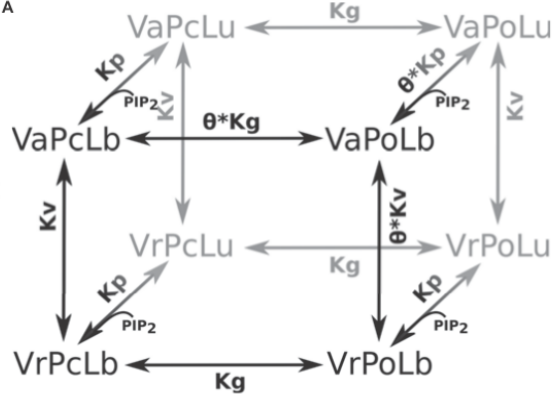
\includegraphics[width=0.4\textwidth]{media/receptor_subunits_half.png}
%      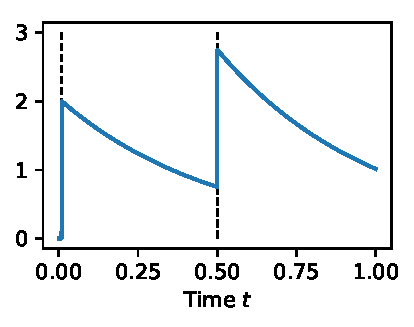
\includegraphics[width=0.4\textwidth]{media/synaptic_filter.pdf}}
%    \end{itemize}
%    \vspace{0.25cm}
%    \emph{Ignores:} physical space, fast dynamics (rise times), adaptation (neurotransmitter depletion)
%\end{frame}

%
%\begin{frame}{Electrophysiological Dynamics --- \emph{Biophysics}}
%	\centering
%	\includegraphics<1>{media/cable_propagation_00.pdf}%
%	\includegraphics<2>{media/cable_propagation_01.pdf}%
%	\includegraphics<3>{media/cable_propagation_02.pdf}%
%	\includegraphics<4>{media/cable_propagation_03.pdf}%
%% \centering{How do neurons process synaptic inputs and transmit them onwards?}
%	% membrane voltage <--> ion channel dynamics
%    % spatial dependence
%    	% - dendritic tree ?=> nonlinear computation of synaptic inputs?
%        % - soma/axon hillock ==> integration (leaky)
%        % - axon ==> creation and propagation of uniform signal
%\end{frame}

%\begin{frame}{Electrophysiological Dynamics --- \emph{Compartmental Models}}
%	Mathematical formalism
%    \begin{itemize}
%      \item cell geometry $\Rightarrow$ segments of electrical cable
%      \pause
%      \item electrodynamics
%      \begin{itemize}
%      	\item between segments $\Rightarrow$ cable equation ($\frac{r_m}{r_l} \frac{\partial^2 V}{\partial x^2} = c_m r_m \frac{\partial V}{\partial t} + V$)
%        \item within segments $\Rightarrow$ system of ODEs for voltage-gated ion channels
%        \pause
%        \end{itemize}
%    \end{itemize}
%    \pause
%    \vspace{1cm}
%    Considerations
%    \begin{itemize}
%      \item accuracy $\propto$ compartments, ion channels, $dt$
%      \item cell-specific
%    \end{itemize}
%\end{frame}

% Section: NEF vs. HBP
\begin{frame}{Comparing LIF and Biology}
  \renewcommand{\arraystretch}{1.5}
  \centering
  \relscale{0.85}\begin{tabular}{r c c r c c}
  	\toprule
  		\multicolumn{3}{c}{\textbf{\textsc{Complexity}}} & \multicolumn{3}{c}{\textbf{\textsc{NEF compatibility}}}\\
  		\cmidrule(r){1-3}\cmidrule(l){4-6}
		& \emph{LIF} & \emph{BIO} & & \emph{LIF} & \emph{BIO} \\
		\cmidrule(r){1-1}\cmidrule(r){2-2}\cmidrule(r){3-3}\cmidrule(lr){4-4}\cmidrule(r){5-5}\cmidrule(l){6-6}
		\textbf{Geometry} & point & compartmental & \textbf{Tuning curve} & $A=f(\mathbf{x})$ & $A=f(\mathbf{x}, t)$ \\
		\textbf{Synapse} & current & conductance & \textbf{Inputs} & linear filter & synaptic nonlinearity \\
		\textbf{Dynamics} & integrate, leak & ion channels & \textbf{Dynamics} & synapse dominates & neuron dominates \\
				 & voltage reset & cable equation & \textbf{Decoders} & static & time-dependent \\
		\textbf{Simulation} & fast & slow & \textbf{Estimates} & $\sum_j a_i(t) * \mathbf{d}_i^f$ & ? \\
  	\bottomrule
  \end{tabular}
\end{frame}

%\begin{frame}{NEF compatibility: \emph{LIF vs. BIO}}
%\begin{table}
%\renewcommand{\arraystretch}{2}
%\begin{tabular}{l || c | c }
% & LIF & BIO \\
%\hline \hline
%Tuning Curve & 
%% Tuning Curve & $a_i^{-1} = \tau_{ref}-\tau_{rc} \log(1 - \frac{J_{thr}}{J_{in}})$ & adaptation \\
%Inputs & linear sum of filtered spikes & spike timing thru synapse \\
%\pause
%Dynamics & synapse dominates & neuron model dominates \\
%\pause
%Decoders & static evaluation points & time-dependent \\
%%\pause
%%Estimates & $\mathbf{\hat{x}}(t) = \sum_j a_i(t) * \mathbf{d}_i^f$ & ? \\
%\end{tabular}
%% \caption{NEF Compatibility}
%\end{table}\end{frame}

\begin{frame}[noframenumbering,plain]
\centering
\Large\textsc{PART II}\\[0.5cm]
{\huge\color{violet}Conductance-based $n$-LIF neurons}
\end{frame}

\begin{frame}{Reversal potentials}
	\centering
	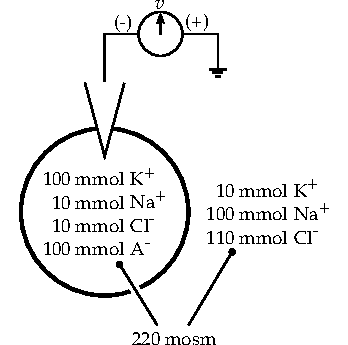
\includegraphics[width=0.35\textwidth]{media/neuron_channel_a.pdf}\hspace{1cm}
	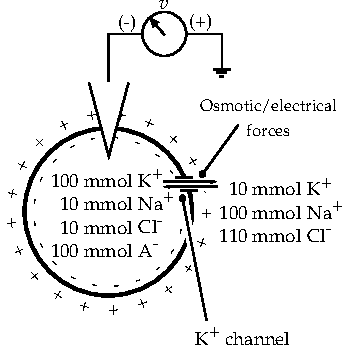
\includegraphics[width=0.35\textwidth]{media/neuron_channel_b.pdf}\\[0.25cm]
	{\color{aluminium4}\footnotesize Illustration adapted from Reichert, 2000, Neurobiology.}\\[0.5cm]
	Ion channels possess a specific \emph{reversal potential} corresponding to the\\
	combination of \emph{ion species} they are permeable for.
\end{frame}

\begin{frame}{Current vs. Conductance-Based LIF}
	\centering
	\begin{columns}
		\column{0.5\textwidth}
		\centering
		\emph{Current-based LIF}\\[0.5cm]
		\begin{overlayarea}{\textwidth}{0.35\textheight}
			\centering
			\includegraphics<1>[width=0.9\textwidth]{media/equivalent_circuit_a.pdf}
			\includegraphics<2>[width=0.5\textwidth]{media/n_comp_lif_a.pdf}
			\includegraphics<3>[width=0.5\textwidth]{media/n_comp_lif_a_b.pdf}
		\end{overlayarea}
		\begin{overlayarea}{\textwidth}{0.25\textheight}
			\only<1-2>{\begin{align*}
				C_\mathrm{m} \dot u(t) &=
					               J^\mathrm{bias} \\
					&           +  \alpha J^\mathrm{syn}(t) \\
					&           +  g_\mathrm{L} (E_\mathrm{L} - u(t))
			\end{align*}}
			\only<3>{\begin{align*}
				C_\mathrm{m} \dot u(t) &=
				J^\mathrm{bias} \\
				&           +  \alpha \big(J^+(t) - J^-(t)\big) \\
				&           +  g_\mathrm{L} (E_\mathrm{L} - u(t))
			\end{align*}}
		\end{overlayarea}
		\column{0.5\textwidth}
		\centering
		\emph{Conductance-based LIF}\\[0.5cm]
		\begin{overlayarea}{\textwidth}{0.35\textheight}
			\centering
			\includegraphics<1>[width=0.9\textwidth]{media/equivalent_circuit_b.pdf}
			\includegraphics<2->[width=0.5\textwidth]{media/n_comp_lif_b.pdf}
		\end{overlayarea}
		\begin{overlayarea}{\textwidth}{0.25\textheight}
			\begin{align*}
	            C_\mathrm{m} \dot u(t) &=
				                   g_\mathrm{E}(t)    (E_\mathrm{E}    - u(t)) \\
				    &           +  \; g_\mathrm{I}(t) (E_\mathrm{I} \; - u(t)) \\
				    &           +  \; g_\mathrm{L} (E_\mathrm{L} \, - u(t))
			\end{align*}
		\end{overlayarea}
	\end{columns}	
\end{frame}

\begin{frame}{Current vs. Conductance-Based LIF Tuning Curves}
	\includegraphics<1>{media/spike_rate_comparison_00.pdf}
	\includegraphics<2>{media/spike_rate_comparison_01.pdf}
	\includegraphics<3>{media/spike_rate_comparison_02.pdf}
\end{frame}

\begin{frame}{Single-compartment conductance-based LIF}
	\begin{itemize}
		\item For firing rates $\gg 0$, conductance-based LIF is boring
	\end{itemize}

	{\centering
	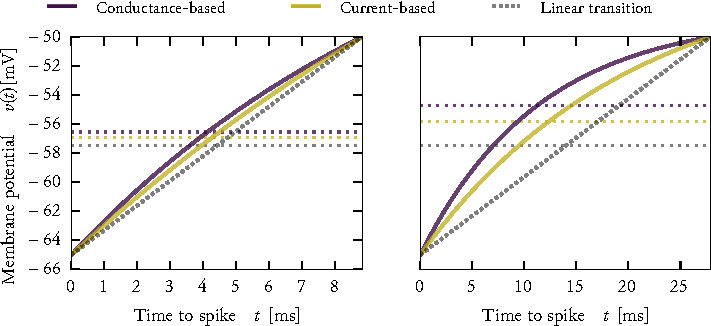
\includegraphics[width=0.75\textwidth]{media/neuron_transitions_cond_vs_cur.pdf}\\}
	\begin{itemize}
		\item Can assume average membrane potential $\bar u$ \only<3->{\emph{$\Rightarrow$} just a skewed current-based LIF!}
		\begin{overlayarea}{\textwidth}{1cm}
		\only<1>{$$
			C_\mathrm{m} \dot u(t) =
			g_\mathrm{E}(t) (E_\mathrm{E}    - u(t))
			+  g_\mathrm{I}(t) (E_\mathrm{I} \; - u(t))
			+  g_\mathrm{L} (E_\mathrm{L} \, - u(t))
			$$}
		\only<2>{$$
			C_\mathrm{m} \dot u(t) =
			g_\mathrm{E}(t) (E_\mathrm{E}    - \bar u)
			+  g_\mathrm{I}(t) (E_\mathrm{I} \; - \bar u)
			+  g_\mathrm{L} (E_\mathrm{L} \, - u(t))
			$$}
		\only<3->{$$
			C_\mathrm{m} \dot u(t) =
			g_\mathrm{E}(t) \alpha_\mathrm{E}
			+  g_\mathrm{I}(t) \alpha_\mathrm{I}
			+  g_\mathrm{L} (E_\mathrm{L} \, - u(t))
			$$}
	\end{overlayarea}
	\end{itemize}
\end{frame}

\begin{frame}{Challenges and Extending the NEF}
	\begin{itemize}
		\setlength{\itemsep}{0.5cm}
		\item<1-> \textbf{Challenges}
		\begin{itemize}
			\setlength{\itemsep}{0.25cm}
			\item[❶]<2->  NEF assumes a constant \emph{bias current}\\
			\emph{$\Rightarrow$} Reinterpretation of tuning curves; optimize weights in \emph{current-space}
			\item[❷]<3-> NEF does not distinguish between \emph{excitatory and inhibitory weights}\\
			\emph{$\Rightarrow$} Solve \emph{non-negative} optimization problems
		\end{itemize}
		\item<4-> \textbf{Extensions}
		\begin{itemize}
			\setlength{\itemsep}{0.25cm}
			\item[❸]<5-> Account for \emph{sub-threshold currents} in the optimization process
			\item[❹]<6-> Take \emph{dendritic non-linearity} into account
		\end{itemize}
	\end{itemize}
\end{frame}

\begin{frame}{❶ Eliminating the Bias Current}
	\centering
	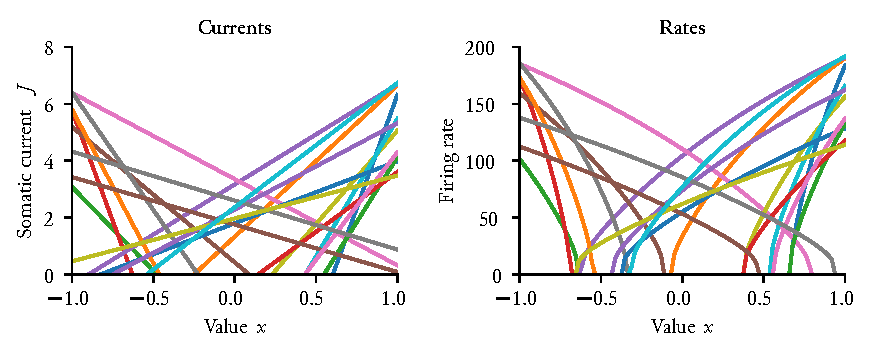
\includegraphics[width=0.9\textwidth]{media/tuning_curves_currents.pdf}

	\begin{overlayarea}{\textwidth}{2cm}
		\begin{itemize}
			\item<2-> Interpret tuning curve as normative: \enquote{We \emph{want} firing rate $a$ if the neuron represents $x$}
			\item<3-> Firing rates correspond to a current $J$: \enquote{We \emph{want} a current $J$ if the neuron represents $x$}
			\item<4->[$\Rightarrow$] Find a current-decoder for \only<4>{each individual post-neuron}\only<5->{\fcolorbox{aluminium5}{aluminium5}{\color{white}\textbf{each individual post-neuron}} (instead of population-wise)}
		\end{itemize}
	\end{overlayarea}
\end{frame}

\begin{frame}{❷ Nonnegative Weight Optimization}
	\begin{itemize}
		\item Assume a post-neuron receives both excitatory and inhibitory input\\
		     from each pre-neuron $i$ \emph{$\Rightarrow$} weight vectors $\vec w_i^+$, $\vec w_i^-$.
	\end{itemize}

	\begin{align*}
	\begin{aligned}
	\min_{\vec w_i^+, \vec w_i^-} &~\hphantom{=\,} \frac{1}2 \sum_{k=1}^N \big\| \vec w_i^+\!\vec a_k^+ - \vec w_i^-\!\vec a_k^- - J\big(\langle \vec e_i, f(\vec x_k)\rangle\big) \big\|_2^2 \\
	&= \frac{1}2 \big\| \vec w_i'\!A' - \vec \jmath \big\|_2^2 \quad\text{where } \vec w_i' = (\vec w_i^+, \vec w_i^-\big),\, A' =  (A^+, -A^-\big)^T,\\&~ \hspace{4.625cm} \text{and } (\vec \jmath)_k = J\big(\langle \vec e_i, f(\vec x_k)\rangle\big) \,, \\
	\text{subject to} &~ \vec w_i^+ \geq 0, \vec w_i^- \geq 0
	\end{aligned}
	\end{align*}
	\vspace{0.25cm}
	\begin{itemize}
		\item Can remove rows/columns from $A'$ and $\vec w_i$ to account for Dale's principle (e.g.~only 20\% of pre-neurons are inhibitory, 80\% are excitatory)
	\end{itemize}
\end{frame}

\begin{frame}{❸ Account for sub-threshold currents}
	\begin{itemize}
		\item Tuning curves are not injective (one-to-one): multiple $x$ map onto a zero output rate
		\item[$\Rightarrow$] If the target rate is zero, we do not care about the current, as long as the rate is zero
		\item[$\Rightarrow$] Turn zero-rates into inequality instead of equality constraints (quadratic programming)
	\end{itemize}
	\centering
	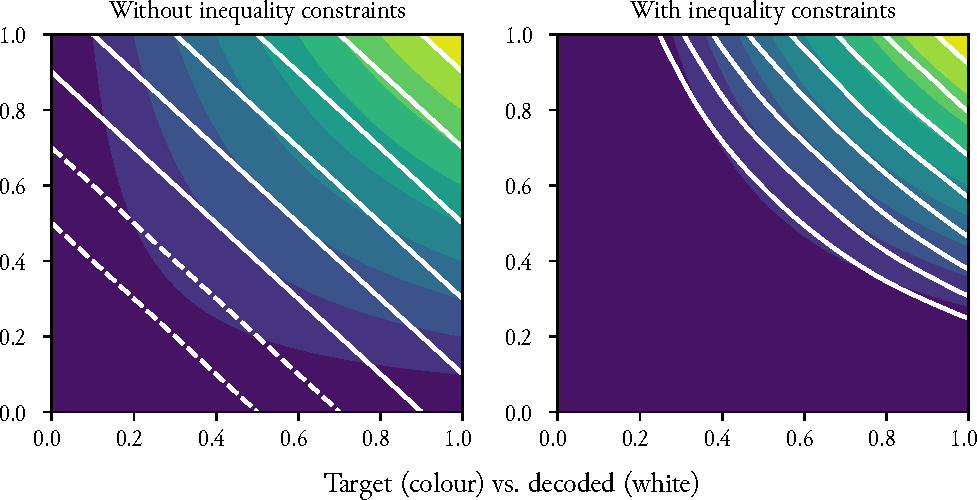
\includegraphics[width=0.75\textwidth]{media/mask_negative.pdf}
\end{frame}

\begin{frame}{❹ Take \emph{dendritic nonlinearity} into account}
	\begin{itemize}
		\setlength{\itemsep}{0.25cm}
		\item Generalise dendritic interaction between excitation and inhibition
		\item Dendritic nonlinearity $H$ converts synaptic state to somatic current
		\item<2-> \textbf{Example:}\\
			\emph{Current-based model:} $H(J^+, J^-) = J^+ - J^-$
			\begin{align*}
			\begin{aligned}
			\min_{\vec w_i^+, \vec w_i^-} &~\hphantom{=\,} \frac{1}2 \sum_{k=1}^N \big\| H( \vec w_i^+\!\vec a_k^+, \vec w_i^-\!\vec a_k^-) - J\big(\langle \vec e_i, f(\vec x_k)\rangle\big) \big\|_2^2 \\
			\text{subject to} &~ \vec w_i^+ \geq 0, \vec w_i^- \geq 0
			\end{aligned}
			\end{align*}
		\item<3-> \textbf{Questions:}
		\begin{itemize}
			\item Can we find more interesting $H$?
			\item Can we exploit $H$ as a computational resource?
			\item Under which conditions can we efficiently solve the optimization problem?
		\end{itemize}
	\end{itemize}
\end{frame}

\begin{frame}{Computing Multivariate Nonlinear Functions}
	\centering
	\raisebox{1.1cm}{\textbf{(A)}}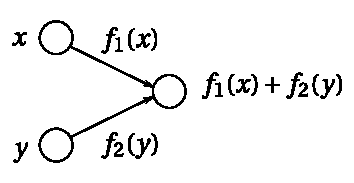
\includegraphics[width=0.35\textwidth]{media/network_a.pdf}\hspace{1cm}
	\raisebox{1.1cm}{\textbf{(B)}}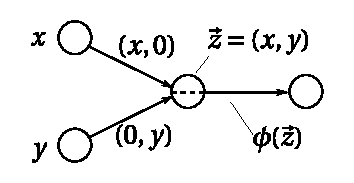
\includegraphics[width=0.35\textwidth]{media/network_b.pdf}
	\raisebox{1.1cm}{\textbf{(C)}}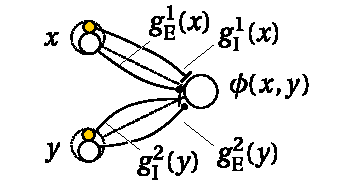
\includegraphics[width=0.35\textwidth]{media/network_c.pdf}\\[0.5cm]
	\emph{Example:} Multiplication, compute $\phi(\vec z) = \phi(x, y) = x \cdot y$
\end{frame}

\begin{frame}{Two-compartment LIF neuron}
	{\centering
	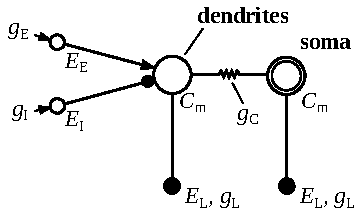
\includegraphics[width=0.35\textwidth]{media/n_comp_lif_c.pdf}\hspace{0.75cm}
	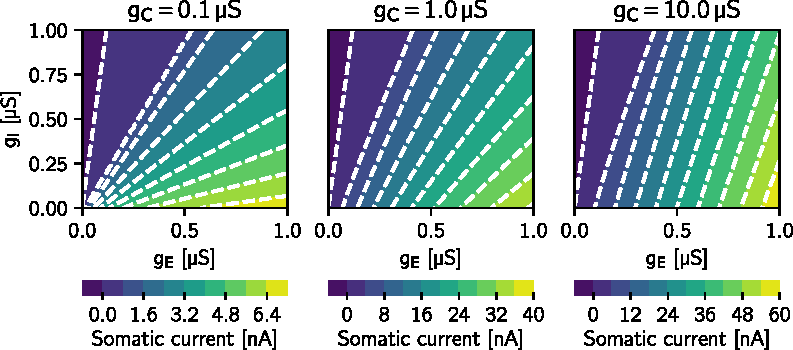
\includegraphics[width=0.55\textwidth]{media/coupling_conductance_linearity_small.pdf}\\}

	\begin{itemize}
		\item Dendritic nonlinearity:
		$$H(g_\mathrm{E}, g_\mathrm{I}) = \frac{b_1 + b_2 g_\mathrm{E} + b_3 g_\mathrm{I}}{a_1 + a_2 g_\mathrm{E} + a_3 g_\mathrm{I}}$$\\[0.25cm]
		\item<2-> Can still formalize weight-optimization as convex quadratic programming problem, guaranteed to find global optimum
	\end{itemize}
\end{frame}

\begin{frame}{Results -- \emph{Dendritic computation} (I)}
	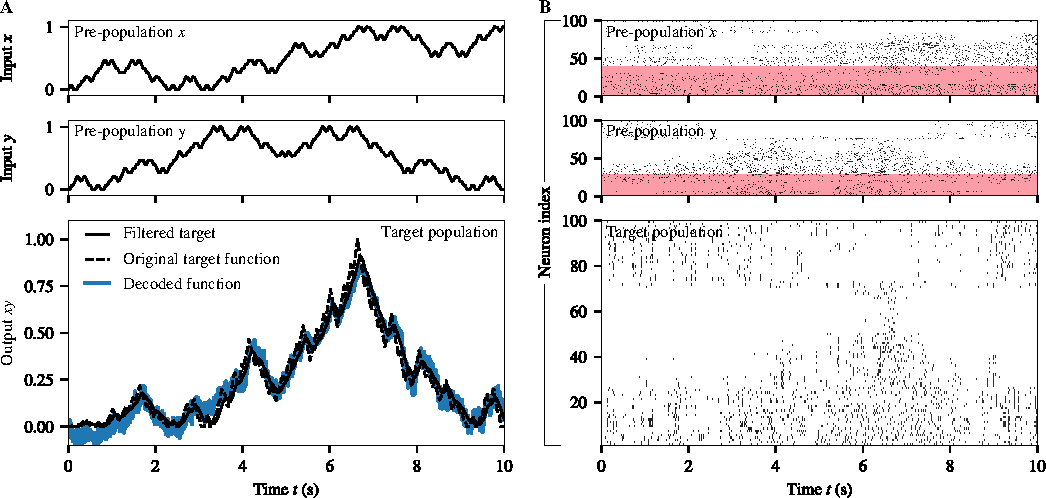
\includegraphics[width=\textwidth]{media/results_example.pdf}
\end{frame}

\begin{frame}{Results -- \emph{Dendritic computation} (II)}
	\centering
	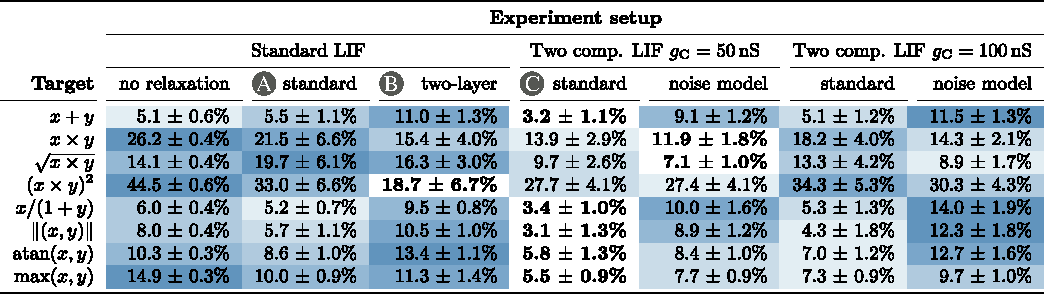
\includegraphics[width=\textwidth]{media/result_table.pdf}\\[0.5cm]
	\url{http://arxiv.org/abs/1904.11713}
\end{frame}

\begin{frame}{Three-compartment LIF neuron}
	\begin{columns}
		\column{0.5\textwidth}
		{\centering
		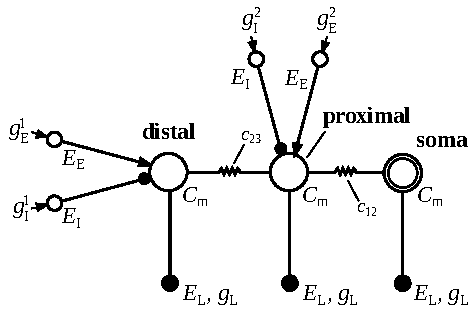
\includegraphics[width=0.66\textwidth]{media/n_comp_lif_d.pdf}\\}
		\begin{itemize}
			\item Dendritic nonlinearity:
			$$\left( \frac{b^1_1 + b^1_2 g_\mathrm{E} + b^1_3 g_\mathrm{I}}{a^1_1 + a^1_2 g_\mathrm{E} + a^1_3 g_\mathrm{I}} \right) \cdot
			  \left( \frac{b^2_1 + b^2_2 g_\mathrm{E} + b^2_3 g_\mathrm{I}}{a^2_1 + a^2_2 g_\mathrm{E} + a^2_3 g_\mathrm{I}} \right)
			$$\\[0.25cm]
			\item<2-> For $n$-LIF, $n \geq 3$: can formalize weight-optimization as iterative trust-region-based optimization problem; \emph{not} guaranteed to find global optimum
		\end{itemize}
		\column{0.5\textwidth}
		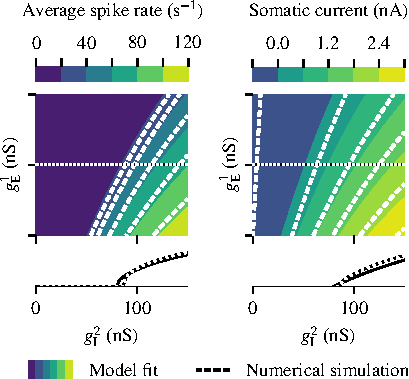
\includegraphics[width=\textwidth]{media/three_compartment_nonlinearity.pdf}
	\end{columns}
\end{frame}

\begin{frame}{Three-compartment LIF neuron -- \emph{Example}}
%	\includegraphics<1>[width=\textwidth]{media/01_multi_comp_iterative.pdf}%
	\includegraphics<1>[width=\textwidth]{media/02_multi_comp_iterative.pdf}%
	\includegraphics<2>[width=\textwidth]{media/03_multi_comp_iterative.pdf}%
	\includegraphics<3>[width=\textwidth]{media/04_multi_comp_iterative.pdf}%
	\includegraphics<4>[width=\textwidth]{media/05_multi_comp_iterative.pdf}%
	\includegraphics<5>[width=\textwidth]{media/06_multi_comp_iterative.pdf}%
	\includegraphics<6>[width=\textwidth]{media/07_multi_comp_iterative.pdf}%
	\includegraphics<7>[width=\textwidth]{media/08_multi_comp_iterative.pdf}%
	\includegraphics<8>[width=\textwidth]{media/09_multi_comp_iterative.pdf}%
	\includegraphics<9>[width=\textwidth]{media/10_multi_comp_iterative.pdf}%
\end{frame}


\begin{frame}[noframenumbering,plain]
\centering
\Large\textsc{PART III}\\[0.5cm]
{\huge\color{violet}Detailed Neuron Models and the NEF}
\end{frame}

\begin{frame}{Neural Engineering Framework}
\centering
\begin{columns}
\column{0.3\textwidth}
    state space \\
    % vector \\
    $\mathbf{x}$ \\
\column{0.3\textwidth}
    $\Longleftrightarrow$ \\
\column{0.3\textwidth}
    neuron space \\
    % spikes, PSC \\
    $\text{A}$ \\
\end{columns}
\begin{figure}
    \centering
    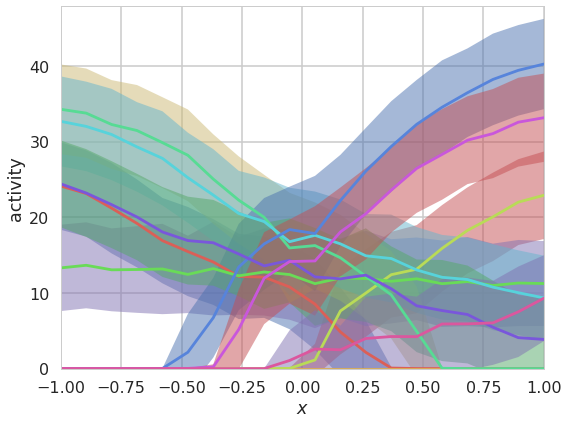
\includegraphics[width=0.85\textwidth]{media/tuning_curves.png}
    \caption{Tuning curves from monkey visual cortex (A) and human NPH (B)} %\cite{eliasmith2012}}
\end{figure}
\end{frame}

\begin{frame}{Problem Statement}
Tuning-curve-based methods assume non-adaptive neurons:
\begin{equation*}
    a_i = F(\mathbf{x})
\end{equation*} \\
\vspace{1cm}
For adaptive neurons, activity depends on signal history
\begin{equation*}
    a_i = F(\mathbf{x}, t)
\end{equation*} \\
\vspace{1cm}
\textbf{Goal}: extend NEF methods to account for cellular dynamics
\end{frame}

%\section{Theory}
\begin{frame}[fragile]{Approach}
Assume neuron model is a ``black box'' \\
\vspace{0.5cm}
Use time-varying signals $\mathbf{x}(t)$ to train neural connection parameters
\begin{itemize}
    \item Encoding: iterative optimization of gain, bias  % $\alpha$, $\beta$
    \item Decoding: least squares optimization of decoders, synapses  % $\mathbf{d}$, $h$
\end{itemize}
\vspace{0.5cm}
Considerations:
\begin{itemize}
    \item $\mathbf{x}(t)$ spans state space and activates appropriate dynamics
    \item $\mathbf{x}(t)$ passes through preliminary filters (spikes, dendrites, etc.)
\end{itemize}
\end{frame}

\begin{frame}[fragile]{Static Encoding}
	Find \texttt{gain} and \texttt{bias} that achieve desired \texttt{max\_rates} and \texttt{intercepts}
	\vspace{0.3cm}
	\begin{columns}
		\column{0.5\textwidth}
		\begin{itemize}
		    \item[1.] Find $J^{\mathrm{test}}(x)$ for $\mathbf{x} \in [-1, 1]$ assuming $\alpha=1$, $\beta=0$ 
		    \item[2.] Calculate $a(J^{\text{test}})$ using rate-approximation
		    \item[3.] Interpolate $a = G(J(\mathbf{x}))$
		    \item[4.] Use $G^{-1}$ to solve for $\alpha$ and $\beta$
		\end{itemize}
		\column{0.5\textwidth}
		\begin{figure}
		    \centering
		    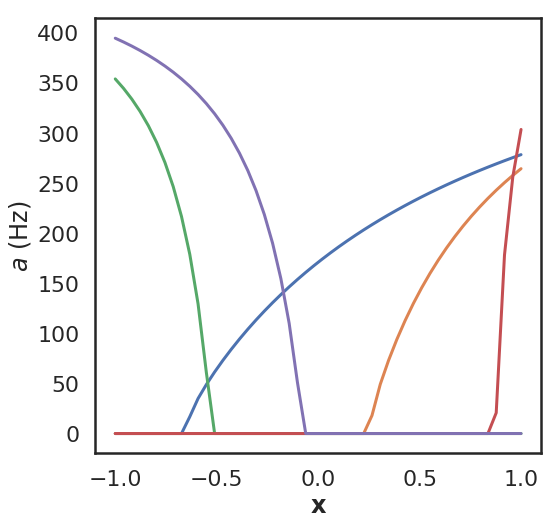
\includegraphics[width=0.5\textwidth]{media/LIF_tuning_default.png}
		\end{figure}
	% \begin{equation}\label{encoding}
	%     J_i(\mathbf{x}) = \alpha_i (\mathbf{e}_i \cdot \mathbf{x}) + \beta_i
	% \end{equation}
	\end{columns}
\end{frame}

\begin{frame}[fragile]{Temporal Encoding}
	Find \texttt{gain} and \texttt{bias} that achieve desired \texttt{max\_rates} and \texttt{intercepts}
	\begin{figure}
	    \centering
	    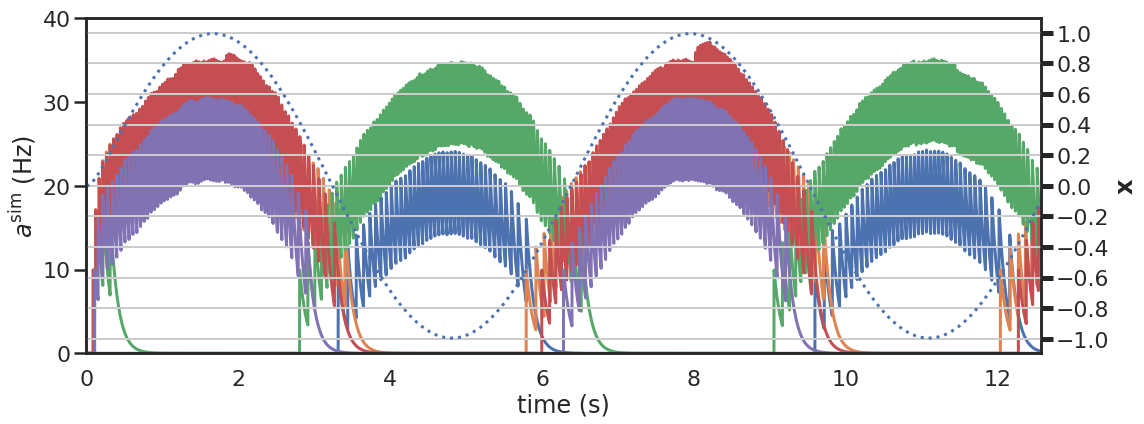
\includegraphics[width=0.8\textwidth]{media/atxt5.png}
	\end{figure}
	\vspace{-0.5cm}
	\begin{figure}
	    \centering
	    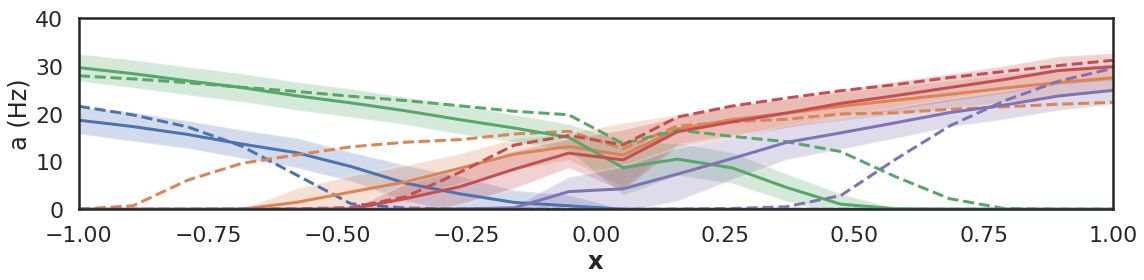
\includegraphics[width=0.8\textwidth]{media/tc1_wide2.png}
	\end{figure}
\end{frame}

\begin{frame}{Static Decoding}
\begin{columns}
	\column{0.5\textwidth}
	\centering
	% Find $\mathbf{d}$ that minimizes the state space error over all $\mathbf{x}$
	Minimizes state-space error over $\mathbf{x}$
	\begin{equation*}
	    E = \frac{1}{2}\int_{-1}^1 (\mathbf{x} - \hat{\mathbf{x}})^2 dx
	\end{equation*}
	\begin{equation*}
	    \hat{\mathbf{x}} = \sum_i a_i ~\mathbf{d}_i
	\end{equation*} \\
	\column{0.5\textwidth}
	Solve using least-squares \\
	\vspace{0.25cm}
	\begin{minipage}{0.5\textwidth}
	\begin{equation*}
	    A ~\mathbf{d} = \mathbf{x}
	\end{equation*}
	\begin{equation*}
	    \mathbf{d} = (A^T A + \sigma^2)^{-1} A^T \mathbf{x}
	\end{equation*}
	\end{minipage}
\end{columns}
\pause
\center{Activity matrix calculated by static encoding}
\begin{equation*}
    A = \begin{bmatrix}
    a_{1}(\mathbf{x}=-1) & \dots & a_{n}(\mathbf{x}=-1) \\
    \vdots & \ddots & \vdots \\
    a_{1}(\mathbf{x}=1) & \dots & a_{n}(\mathbf{x}=1) \\
    \end{bmatrix}
\end{equation*}
\begin{equation*}
    a_i(\mathbf{x}) = G_i(\mathbf{x}, \alpha_i, \beta_i)
\end{equation*}
\end{frame}

\begin{frame}{Temporal Decoding}
\begin{multicols}{2}
\centering
% Find $\mathbf{d}$ that minimizes the state space error over all $t$
Minimize state-space error over $t$
\begin{equation*}
    E = \frac{1}{2}\int_{0}^{t'} (\mathbf{x}(t) - \hat{\mathbf{x}}(t))^2 dt
\end{equation*}
\begin{equation*}
    \hat{\mathbf{x}}(t) = \sum_i a_i(t) ~\mathbf{d}_i
\end{equation*} \\
\columnbreak
Solve using least-squares \\
\vspace{0.25cm}
\begin{minipage}{0.5\textwidth}
\begin{equation*}
    A ~\mathbf{d} = \mathbf{x}(t)
\end{equation*}
\begin{equation*}
    \mathbf{d} = (A^T A)^{-1} A^T \mathbf{x}(t)
\end{equation*}
\end{minipage}
\end{multicols}
\pause
\center{Activity matrix collected by simulating over time}
\begin{equation*}
    A = \begin{bmatrix}
    a_{1}(t=0) & \dots & a_{n}(t=0) \\
    \vdots & \ddots & \vdots \\
    a_{1}(t=t') & \dots & a_{n}(t=t') \\
    \end{bmatrix}
\end{equation*}
\begin{equation*}
    \mathbf{x}(t) = [\text{computed directly}]
\end{equation*}
\end{frame}

%\section{Results}
\begin{frame}{Neuron Models}
\centering
\begin{multicols}{3}
\textbf{Adaptive LIF} \\
\vspace{0.2cm}
- spikes increase $V^{\text{thr}}$ \\
\vspace{0.1cm}
- divisive effect on $J$ \\
\columnbreak
\textbf{Wilson} \\
\vspace{0.2cm}
- mamalian neocortex \\  %HH-like model of 
\vspace{0.1cm}
- 3 coupled ODEs for \\
$V$, $R$, $C$ \\
% voltage, recovery, conductance \\
\columnbreak
\textbf{Durstewitz} \\
\vspace{0.2cm}
- Layer-V PC \\
- conductance syn. \\
- 4 geo. compartments \\
- 6 HH ion channels \\  % HH formalism w/ 
% \vspace{0.1cm}
% - Da perturbation \\
\end{multicols}
\vspace{-0.2cm}
\begin{figure}
    \centering
    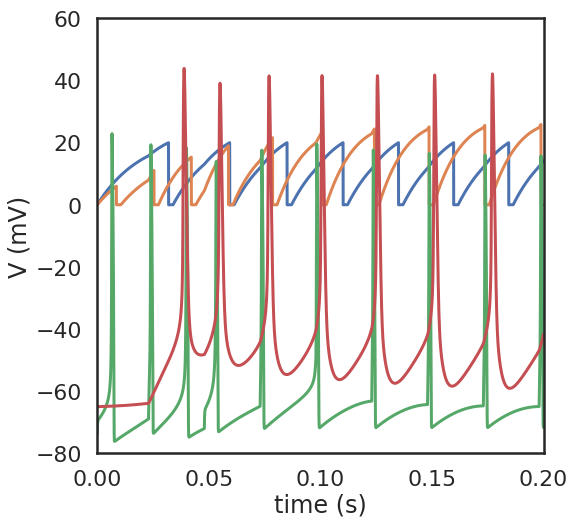
\includegraphics[width=0.35\textwidth]{media/v_compare.png} \hspace{1.5cm}
    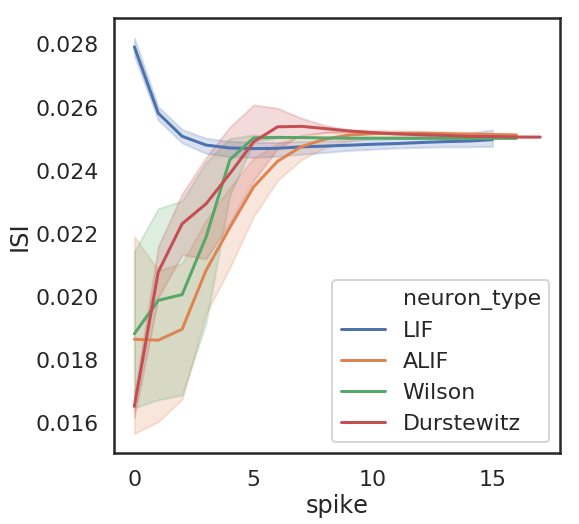
\includegraphics[width=0.35\textwidth]{media/isi_compare.png}
    \caption{Adaptive response to spiking input representing $\mathbf{x}(t)=1$}
\end{figure}
\end{frame}

\begin{frame}{Encoding: Training $\alpha$ and $\beta$}
\only<1>{
    \begin{figure}
    \centering
    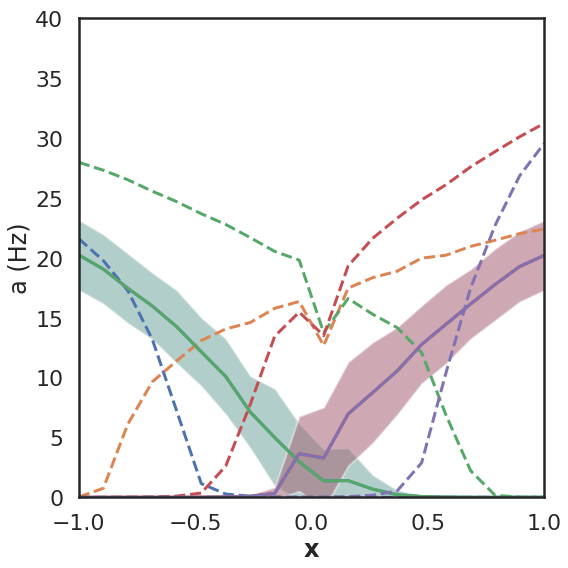
\includegraphics[width=0.55\textwidth]{media/tc0.png}
    \caption{Tuning curves before training}
    \end{figure}}
\only<2>{\begin{figure}
    \centering
    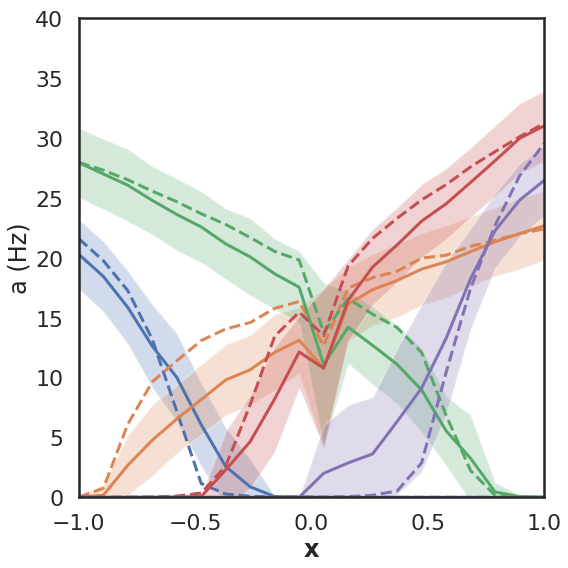
\includegraphics[width=0.55\textwidth]{media/tc9.png}
    \caption{Tuning curves after training}
    \end{figure}}
\end{frame}

\begin{frame}{Decoding: $f(x) = x$}
\begin{figure}
    \centering
    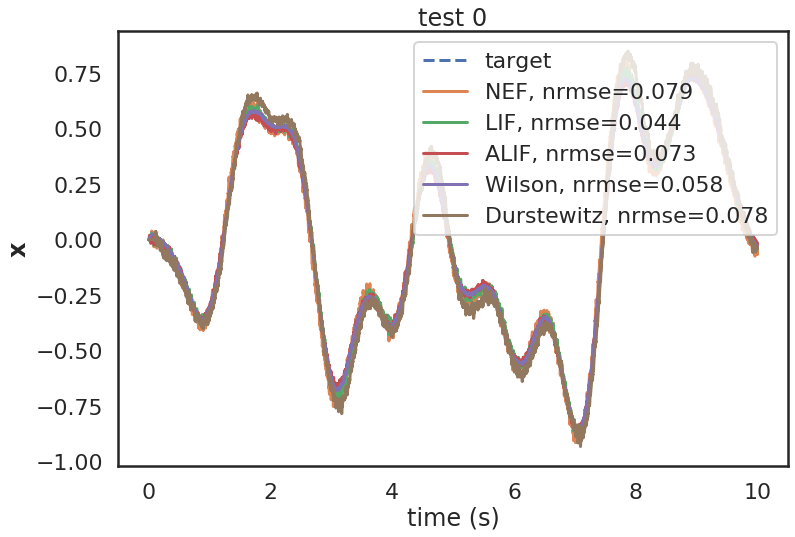
\includegraphics[width=0.8\textwidth]{media/feedforward_test0_order1.png}
    \caption{Decoded activities of $100$ neurons driven with filtered white noise}
\end{figure}
\end{frame}
\begin{frame}{Decoding: $f(x) = x$}
\begin{figure}
    \centering
    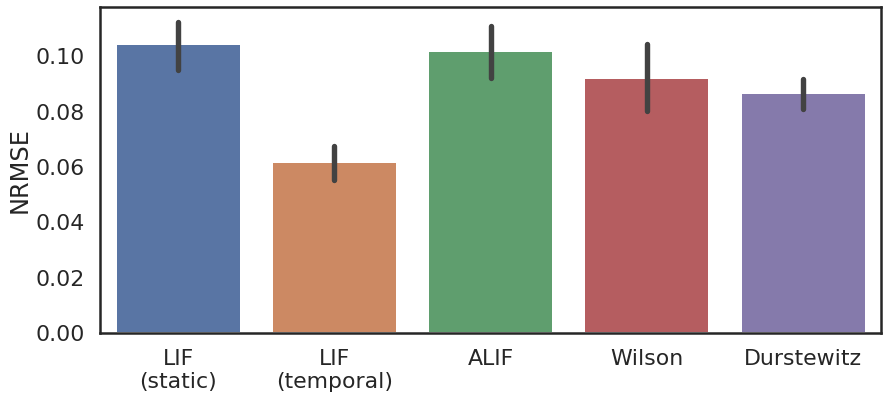
\includegraphics[width=0.8\textwidth]{media/feedforward_barplots_order1.png}
    \caption{Average performance across neuron models}
\end{figure}
\end{frame}

\begin{frame}{Decoding: $f(x) = x^2$}
\begin{figure}
    \centering
    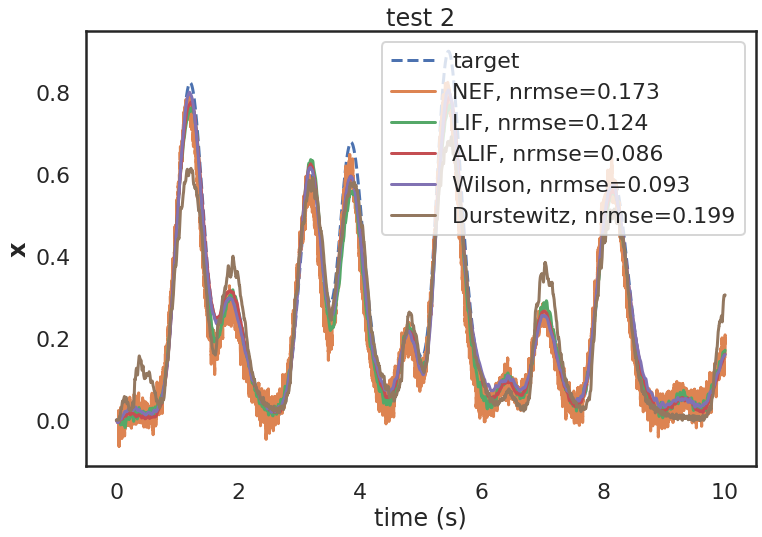
\includegraphics[width=0.8\textwidth]{media/function_test2_order2.png}
    \caption{Decoded activities of $100$ neurons driven with filtered white noise}
\end{figure}
\end{frame}
\begin{frame}{Decoding: $f(x) = x^2$}
\begin{figure}
    \centering
    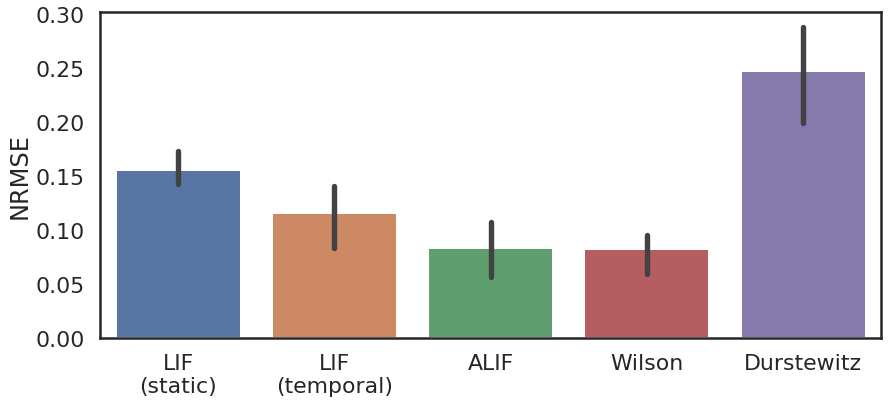
\includegraphics[width=0.8\textwidth]{media/function_barplots_order2.png}
    \caption{Average performance across neuron models}
\end{figure}
\end{frame}

\begin{frame}{Dynamical System: 2D Oscillator}
\begin{figure}
    \centering
    %\includegraphics[width=0.9\textwidth]{media/oscillator.png}
    \caption{Implementing a two-dimensional oscillator using $200$ recurrently-connected neurons}
\end{figure}
\end{frame}

\begin{frame}{Dynamical System: Lorenz Attractor}
\begin{figure}
    \centering
    %\includegraphics[width=0.9\textwidth]{media/oscillator.png}
    \caption{Implementing a three-dimensional chaotic attractor using $2000$ recurrently-connected neurons}
\end{figure}
\end{frame}


\begin{frame}{Future Work}
\textbf{Nengo Integration}
\begin{itemize}
    \item Online learning
    % \item SPA
\end{itemize}
\vspace{0.5cm}
\textbf{Applications}
\begin{itemize}
    \item Harder dynamics
    \item Cognitive models
    \item Drug effects
\end{itemize}
\vspace{0.5cm}
\textbf{Extensions}
\begin{itemize}
    \item Dale's principle
    \item Functional neuromodulation
\end{itemize}
\end{frame}

%\section{Conclusion}
\begin{frame}{Summary}
Training $\alpha$, $\beta$ using $\mathbf{x}(t)$ distributes tuning curves of complex neurons \\
\vspace{0.5cm}
Training $\mathbf{d}$ using $\mathbf{x}(t)$ decodes activities of adaptive neurons \\
\vspace{0.5cm}
Training $h(t)$ using $\mathbf{x}(t)$ controls for cell dynamics in recurrent networks \\
\vspace{0.5cm}
\rule{\textwidth}{1pt}
% \hline
\center{Thanks to \\
\vspace{0.5cm}
\textbf{Aaron Voelker} ~~Terry Stewart ~~Andreas St\"{o}ckel ~~Chris Eliasmith} \\
\end{frame}

\begin{frame}[noframenumbering,plain]
\centering
\Large\textsc{PART IV}\\[0.5cm]
{\huge\color{violet}\texttt{nengo-bio} hands-on}
\end{frame}

%\begin{frame}[noframenumbering,plain]
%\centering
%\Large\textsc{PART V}\\[0.5cm]
%{\huge\color{violet}Summary \& Conclusion}
%\end{frame}
%
%\begin{frame}{Summary}
%	\begin{itemize}
%		\setlength{\itemsep}{0.5cm}
%		\item<1-> Modelling with biologically plausible neurons is interesting for a variety of reasons
%		\item<2-> Conductance-based synapses can be integrated into the NEF and increase the computational power per neuron
%		\item<3-> Arbitrarily complex neuron models can be substituted into Nengo\\networks with mixed success (so far)
%	\end{itemize}
%
%	\begin{overlayarea}{\textwidth}{0.25\textheight}
%	\only<5->{
%	\Huge
%	\centering
%	{\color{aluminium3}}
%
%	Thank you for your attention!}
%	\end{overlayarea}
%\end{frame}

\backupbegin

\backupend

\end{document}
